% NIME 2020 Music Proceedings Template

% Modified December 2019 by Joe Wright
% Created August 2019 by Niccolo Granieri
% This is file `music-proceedings-template.tex',
%
% The original source files were:
%
% samples.dtx  (with options: `acmsmall')
% 
% IMPORTANT NOTICE:
% 
% For the copyright see the source file.
% 
% Any modified versions of this file must be renamed
% with new filenames distinct from sample-acmsmall.tex.
% 
% For distribution of the original source see the terms
% for copying and modification in the file samples.dtx.
% 
% This generated file may be distributed as long as the
% original source files, as listed above, are part of the
% same distribution. (The sources need not necessarily be
% in the same archive or directory.)


% The first command in your LaTeX source must be the 
% \documentclass command.
\documentclass{nimemusic}


\usepackage{lipsum} %used to generate default text
% Rights management information.  This information is sent to you
% when you complete the rights form.  These commands have SAMPLE
% values in them; it is your responsibility as an author to replace
% the commands and values with those provided to you when you
% complete the rights form.
\setcopyright{cc4}
\nimeYear{2024}
\nimeMonth{9}
\nimeDOI{10.1145/XXXXXXX.XXXXXXX}
\whichNIME{NIME’24, 4--6 September, 2024, Utrecht, The Netherlands}

%\fancypagestyle{firstPage}{%
%  \fancyhf{}
%  \renewcommand\headrulewidth{0pt}
%  \fancyfoot[R]{Some special text}
%}


% end of the preamble, start of the body of the document source.
\begin{document}

% The "title" command has an optional parameter,
% allowing the author to define a "short title" to be used in page headers.
\title{Title: Your NIME Music Performance}



% The "author" command and its associated commands are used to define
% the authors and their affiliations.
% Of note is the shared affiliation of the first two authors, and the
% "authornote" and "authornotemark" commands
% used to denote shared contribution to the research.
\author{Author \#1}
\affiliation{%
  \institution{Affilitation \#1}
  \city{City}
  \country{Country}
}

\author{Author \#2}
\affiliation{%
  \institution{Affilitation \#1}
  \city{City}
  \country{Country}
}

\author{Author \#3}
\affiliation{%
  \institution{Affilitation \#1}
  \city{City}
  \country{Country}
}


% By default, the full list of authors will be used in the page
% headers. Often, this list is too long, and will overlap
% other information printed in the page headers. This command allows
% the author to define a more concise list
% of authors' names for this purpose.
\renewcommand{\shortauthors}{Trovato and Tobin, et al.}


% Keywords. The author(s) should pick words that accurately describe
% the work being presented. Separate the keywords with commas.
\keywords{datasets, neural networks, gaze detection, text tagging}


% This command processes the author and affiliation and title
% information and builds the first part of the formatted document.
\maketitle
%\thispagestyle{firstPage}


\section{Program Notes}
\lipsum[1] Plus, some citations to articles: \cite{bowman:reasoning,
clark:pct, braams:babel, herlihy:methodology}.

\begin{figure}[hbt]
  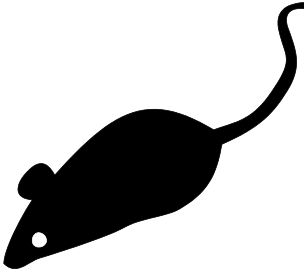
\includegraphics{NIME_Mouse}
  \caption{The NIME Mouse}
\end{figure}


\section{Project Description}
\lipsum[2]

\section{PERFORMANCE NOTES}
\lipsum[3]

\section{Media Links}

\begin{itemize}
	\item Video: \url{www.yournimevideolink.com/younameit}
	\item Audio: \url{www.yournimeaudiolink.com/younameit}
\end{itemize}


% The acknowledgments section is defined using the "acks" environment
% (and NOT an unnumbered section). This ensures the proper
% identification of the section in the article metadata, and the
% consistent spelling of the heading.
\begin{acks}
The authors would like to thank...
\\
This work was supported by...
\end{acks}

\section*{Ethical Standards}
Please note, that if any elements of the submitted work involve research with people or animals, authors should include a section “Compliance with Ethical Standards” before the References, including (if relevant): information regarding sources of funding, potential conflicts of interest (financial or non-financial),  informed consent if the research involved human participants, statement on welfare of animals if the research involved animals.

% The next two lines define the bibliography style to be used, and
% the bibliography file.
\bibliographystyle{nime-music-references.bst}
\bibliography{nime-references.bib}
\end{document}
\endinput
%
% End of file `sample-acmsmall.tex'.
